\chapter{Produktidee}

\section{Einleitung}

Das effektive und vorallem zeit- und energieoptimale Ansteuern von Roboterarmen stellt trotz modernster Rechner, wegen der hohen Problemkomplexität, eine große Herausforderung dar. Es ist bis heute nicht gelungen einen Algorithmus zu entwerfen der diese Problem optimal löst und daher arbeiten alle Anlagen mit Naherungslösungen für die optimale Pfadplanung.

Unsere Idee ist es ein Künstliches Neuronales Netzwerk auf die Lösung dieses Problems zu trainieren um so eine höhere Energieeffizienz und Geschwindigkeit des Roboterarmes zu erreichen.

\section{Umsetzung}

Zur Umsetzung einer Robotersteuerung gibt es grundsätzlich zwei Ansätze. Bei dem ersten Ansatz wird vor dem Losfahren offline eine Trajektorie berechnet welche anschließend als Liste von Punkten zum Roboter übertragen werden welcher diese nacheinander linear angefährt. Der zweite Ansatz ist das Online-planing, hierbei entfällt die Wartezeit vor dem Verfahren und der Roboter versucht sofort, anhand eines Algorithmus, seine Zielposition zu erreichen. 

\begin{figure}[h]
	\centering
	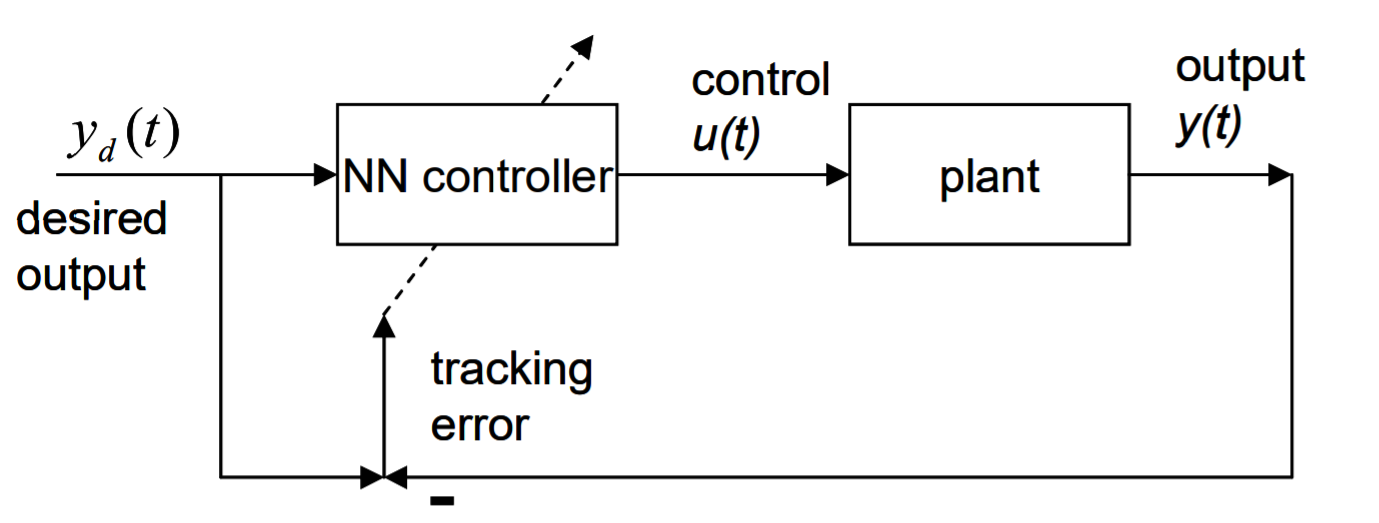
\includegraphics[width=15cm]{NN_controller_system.png}
	\caption{Regelung eines Systems basierend auf einem Neuronalen Netzwerks}
	\label{fig:NeuralNetworkControlSystem}
\end{figure}

Die Vorteile unseres Ansatzes mit einem Neuronalen Netzwerk (NN) liegen darin, dass die Modellbildung durch ein Neuronales Netzwerk sämtliche physikalischen Effekte in der Mechanik des Roboters wie Nichtlineare-Reibung berücksichtigt werden, was mit etablierten Ansätzen nur teilweise möglich ist.

Vorrangegangene Prototypen für eine NN basierte Regelung der Roboterarm-gelenke haben gezeigt, dass Effizienzsteigerungen von bis zu 30\% im Vergleich zu herkömmlichen Algorithmen möglich sind. Die so erzeugten Trajektorien sind nicht nur Energiesparender, sondern auch schonender für die Mechanik, da sie sanfter Beschleunigungs- und Bremsvorgänge  einzelner Gelenke verwenden. Durch die optimierte Trajektorie wird die Gesamtzeit zum Erreichen des Zielpunktes jedoch nicht verlängert, sondern kann in vielen Fällen sogar reduziert werden.

Unser Produkt ist ausschließlich die Software, welche auf der Robotersteuerung läuft und die Regelung übernimmt, und umfasst keine Hardware. Auf diese Weise wollen wir uns voll auf unsere Hauptkompetenz fokussieren.

